\documentclass{beamer}

\usepackage{mathtools}
\usepackage[style=numeric-comp, sorting=none]{biblatex}
\addbibresource{bibliographie.bib}

\title{Synthèse et expériences numériques liées à un article de recherche}
\subtitle{Conductivité thermique négative des \\ chaînes de rotors avec forçage mécanique}

\author[dfrenkiel]{David Frenkiel}
\institute{Cours 5MM50 \\ Sorbonne Université}

\newcommand{\vs}{\vspace{10.0mm}}
\setlength{\parskip}{3.0mm}

\begin{document}

    \begin{frame}
    \titlepage
\end{frame}


    \begin{frame}

    \frametitle{Partie I \\
        Synthèse - Dynamique hors équilibre}

    Synthèse des sections 7.2, 7.3, 7.4, et 7.5 des notes de cours :

    \textbf{Introduction à la physique statistique numérique}
    \cite{stoltz_phys_stat}

    Gabriel Stoltz.

    \small \url{http://cermics.enpc.fr/~stoltz/Cours/intro_phys_stat.pdf}

\end{frame}

\begin{frame}

    \frametitle{Synthèse - Dynamique hors équilibre}

    La dynamique hors équilibre caractérise un système qui n'est pas
    réversible. Physiquement, un tel système présente un flux d'énergie
    (chaleur) d'une partie du système vers une autre.

    Ici, on suscite une dynamique hors équilibre, et donc un flux
    d'énergie, en appliquant au système des forçages thermiques et
    mécaniques.

    Lorsque le gradient de température est faible (et sans forçage),
    le flux reste linéaire, et la loi de Fourier s'en applique. En
    revanche, dès que le gradient de température est plus important,
    la dynamique devient beaucoup plus compliquée. Il n'existe pas
    une théorie générale dans ce cas.

\end{frame}

\begin{frame}

    \frametitle{Synthèse - Dynamique hors équilibre}

    En générale il n'est pas possible de déterminer analytiquement
    la mesure invariante d'un système hors équilibre. En particulier,
    cette mesure dépend des détails de la dynamique d'une manière
    non-triviale à cause des corrélations de longue portée.

    Par exemple, pour la dynamique perturbée,
    %
    \[dq_t = (-V'(q) + F)dt + \sqrt{2} dW_t,\]
    %
    la mesure invariante $\psi_F$ est
    %
    \[\psi_F(q) = Z_F^{-1} \int_0^1 e^{V(q+y) - V(q) -Fy} dy.\]
    %
    Si $F \neq 0$, cette mesure dépend des valeurs de $V$ partout.

\end{frame}



%$$\psi_F(q) = Z_F^{-1} \int_0^1 e^{V(q+y) - V(q) -Fy} dy
%= Z_F^{-1} e^{-V(q)} \int_0^1 e^{V(q+y)} e^{-Fy} dy.$$


%Pour la mesure invariante quand F \neq 0: si on change V qq part,
%l'expression de la mesure invariante (une sorte de convolution)
%montre que la densité change partout, de manière non triviale ;
%
%En contraste avec le cas d'une mesure de Gibbs dont la densité
%est proportionnelle à e^{-\beta V(q)} dq, et donc si on change
%localement la valeur de V, on ne change la densité de la mesure
%que localement (à un facteur de rescaling près).
%
%Le mieux pour vous en convaincre serait de faire une quadrature
%numérique pour calculer \psi_F, de changer V localement
%(pex ajouter un créneau à support petit), et regarder comment
%ça change la mesure globale.





















% calcul flux energie - stoltz page 33
% loi fourier

%    TODO
%    \begin{frame}
%        \frametitle{Calcul coefficients de transport}
%        Flux d'énergie...
%        Température !!!!!!!!!!!!!!!!!!
%    \end{frame}












% A very interesting question is whether nonequilibrium systems
% are locally close to equilibrium.
% c'est quoi ca ?
% file:///Users/frenkield/Library/Mobile%20Documents/com~apple~CloudDocs/cours/cours-spe%CC%81cialise%CC%81s/5MM50-mole%CC%81culaire/slides/rotors-alessandra-Iacobucci.pdf



% Donc... Fokker-Planck est juste l'EDP qui satisfait la mesure.


% sections 7.2 à 7.4 [et j'aurais discuté qq éléments de la section 7.5]


%\begin{frame}
%
%    \frametitle{Dynamique hors équilibre}
%
%    La dynamique hors équilibre caractérise un système qui n'est pas
%
%    \begin{equation}
%        \begin{dcases}
%            dq_{t} = M^{-1} p_{t} d t \\
%            dp_{t} = \left(-\nabla V\left(q_{t}\right) + \eta F\right)
%            dt-\gamma M^{-1} p_{t} d t + \sqrt{\frac{2 \gamma}{\beta}} dW_{t}
%        \end{dcases}
%        \label{eq:dynamique}
%    \end{equation}
%
%    % It is precisely because the perturbation is not of gradient type that
%    % some particle flux can appear in the steady-state.
%
%    % Attaching the chain on one side is important to remove the translation invariance of the whole system.
%
%    % η, and the proportionality constant is called the mobility.
%
%
%    We believe that there exists a unique smooth station-ary measure for the
%    dynamics (2). However, as far as weknow, there is no rigorous result in
%    this direction for ro-tor chains, even in the caseF= 0. Indeed, the
%    standardtechniques (see for instance [11, 12]) used to prove exis-tence
%    and uniqueness of an invariant measure for chainsof oscillators under
%    thermal forcing do not apply here
%
%
%    Some interesting relations can nonetheless be obtainedunder
%    the assumption that the stationary state exists.
%
%
%    % IfF= 0 andTL=TR=T, the system is inequi-librium, and the unique stationary measure is given bythe Gibbs measure
%
%\end{frame}


%
%        The Langevin dynamics may be seen as some modification of the Hamiltonian dynamics with
%        two added components: a damping term −γ(qt)M−1pt dt (dissipation) and a random forcing term
%        σ(qt)dWt (fluctuation). The energy dissipation due to damping is compensated by the random
%
%        stoltz page 33


%Of course, to reach some steady-state, some dissipation
%mechanism has to be considered as well, otherwise the external forcing may
%lead to an uncontrolled growth of the energy of the system.


%    Les propriétés thermodynamiques des états stationnaires hors équilibre
%    sont très peu comprises. Ces états sont généralement caractérisés par

%    des courants de quantités conservées (telles que l’énergie), qui circulent
%    dans le système. Lorsque les états stationnaires sont proches des états
%    d’équilibre, c’est-à-dire quand les perturbations sont de faible intensité,
%    la théorie de la réponse linéaire est efficace et explique les phénomènes
%    macroscopiques communs tels que la loi de Fourier. Ainsi, dans un système
%    en contact avec deux thermostats à températures différentes, si la différence
%    entre les deux températures est faible, le flux de chaleur est proportionnel
%    au gradient thermique. D’autre part, il n’y a pas de théorie générale pour
%    décrire les systèmes dans un état stationnaire loin de l’équilibre, et les
%    propriétés macroscopiques correspondantes semblent dépendre des détails
%    spécifiques de la dynamique.

%    A traditional way to implement the interaction with reservoirs amounts
%to introducing simul-taneously random forces and dissipation according
%to the generalprescription of fluctuation-dissipation theorem. This could
%be regarded as the limit case of the previous model whenγ±becomes very large.
%Consequently, the reservoirs are not affected by the system dynamics. In
%the simple case of an equal-mass chain, this results in the following set
%of Langevin equations

%    \gamma >0 determines the strength of the coupling to the thermostat
% (fluctuation-diffusion).

% In all schemes of heat baths there is at least one parameter controlling
%the coupling strength:let us generically call itg. It can either be the
%inverse of the average time between subsequentcollisions, or the
%dissipation rate λ in the Langevin equation

% https://arxiv.org/pdf/cond-mat/0112193.pdf page 15

% Ornstein-Uehlenbeck process


% Another prototypical feature of the Langevin equation is the occurrence of
%the damping coefficient λ {\displaystyle \lambda } \lambda in the correlation
%function of the random force, a fact also known as Einstein relation.


% For example, Albert Einstein noted in his 1905 paper on Brownian motion
%that the same random forces that cause the erratic motion of a particle
%in Brownian motion would also cause drag if the particle were pulled through
%the fluid. In other words, the fluctuation of the particle at rest has the
%same origin as the dissipative frictional force one must do work against,
%if one tries to perturb the system in a particular direction.

% fluctuation-dissipation


% hors equilibre - constats interressants
% calcul temperature (pdf utile - "energy continuity equation")
% loi fourier
% thermostat
% flux d'energie total
% forcage modelise quoi ???????????? c'est dans un de ces articles......


%    \bibliographystyle{plain}
%    \bibliography{sample}
%    \printbibliography


    \begin{frame}

    \frametitle{Partie II \\ Article de recherche}

    \textbf{Negative thermal conductivity of chains of rotors with mechanical forcing}
    \cite{Iacobucci_2011}

    Alessandra Iacobucci, Frédéric Legoll, Stefano Olla, et Gabriel Stoltz

    \url{https://arxiv.org/abs/1107.1766}

\end{frame}

\begin{frame}

    \frametitle{Article de recherche}

    L'article porte sur le comportement particulier des chaînes de rotors soumises
    aux forçages thermiques et mécaniques. Ce système hors équilibre présente
    quelques propriétés remarquables :

    \begin{itemize}

        \item Des profils non linéaires inhabituels de température et de vitesse

        \item La température est maximale vers le centre de la chaine

        \item Cependant, l'équilibre local se maintient pour des chaînes longues.

        \item Lorsque le forçage mécanique est suffisamment fort, le flux
        d'énergie peut être augmenté par un gradient de \alert{température inverse}.

    \end{itemize}

\end{frame}

    \begin{frame}

    \frametitle{Modèle - Chaîne de rotors}

    Une chaîne de rotors modélise un système unidimensionnel où chaque molécule
    interagit avec ces 2 voisins sous l'influence d'un potentiel périodique.

    Ce modèle s'applique, par exemple, aux rotations des paires de bases de
    l'ADN ou des séries de jonctions Josephson \cite{TAKENO1996140}.

    \begin{itemize}
        \item Position (angle) du rotor $i$ : $q_i \in [0, 2\pi]$
        \item Impulsion du rotor $i$ : $p_i \in \mathbb{R}$
        \item Potentiel : $V = \sum_i 1 - \cos(q_i - q_{i-1})$
    \end{itemize}

\end{frame}







%    Donc la dissipation sert à empecher l'énergie du système de
%    diverger.


    %    A traditional way to implement the interaction with reservoirs amounts
%to introducing simul-taneously random forces and dissipation according
%to the general prescription of fluctuation-dissipation theorem. This could
%be regarded as the limit case of the previous model when γ± becomes very large.
%Consequently, the reservoirs are not affected by the system dynamics. In
%the simple case of an equal-mass chain, this results in the following set
%of Langevin equations

%    \gamma >0 determines the strength of the coupling to the thermostat
% (fluctuation-diffusion).

% In all schemes of heat baths there is at least one parameter controlling
%the coupling strength:let us generically call itg. It can either be the
%inverse of the average time between subsequentcollisions, or the
%dissipation rate λ in the Langevin equation














\begin{frame}

    \frametitle{Modèle - Chaîne de rotors}

    On considère ici une dynamique où la chaîne est soumise aux forces
    thermiques et mécaniques. La masse de chaque rotor est 1.0, et les
    rotors à gauche et à droite sont attachés aux thermostats de
    Langevin.

    Le rotor à gauche est collé à la paroi, tandis que le rotor à
    droite est soumis à une force externe constante.

    En collant le rotor à gauche à la paroi, on retire l'invariance
    par translation du système.

    % \colorbox{green}{Pourquoi c'est important ?}

    % [sans l'invariance par translation] there is no hope of finding an
    % invariant probability measure
    % https://hal.archives-ouvertes.fr/hal-00115627/document

    On verra que la combinaison de ces 2 influences suscite des
    phénomènes surprenants. Par exemple, sous certain conditions,
    l'augmentation de la température à droite \alert{réduit} le flux
    d'énergie vers la gauche.

\end{frame}


\begin{frame}

    \frametitle{Modèle - Chaîne de rotors}

    Une chaîne de rotors (sans forçage) avec des thermostats à
    gauche et à droite. Le rotor à gauche est collé à la paroi.

    \begin{figure} % [H]
        \centering
        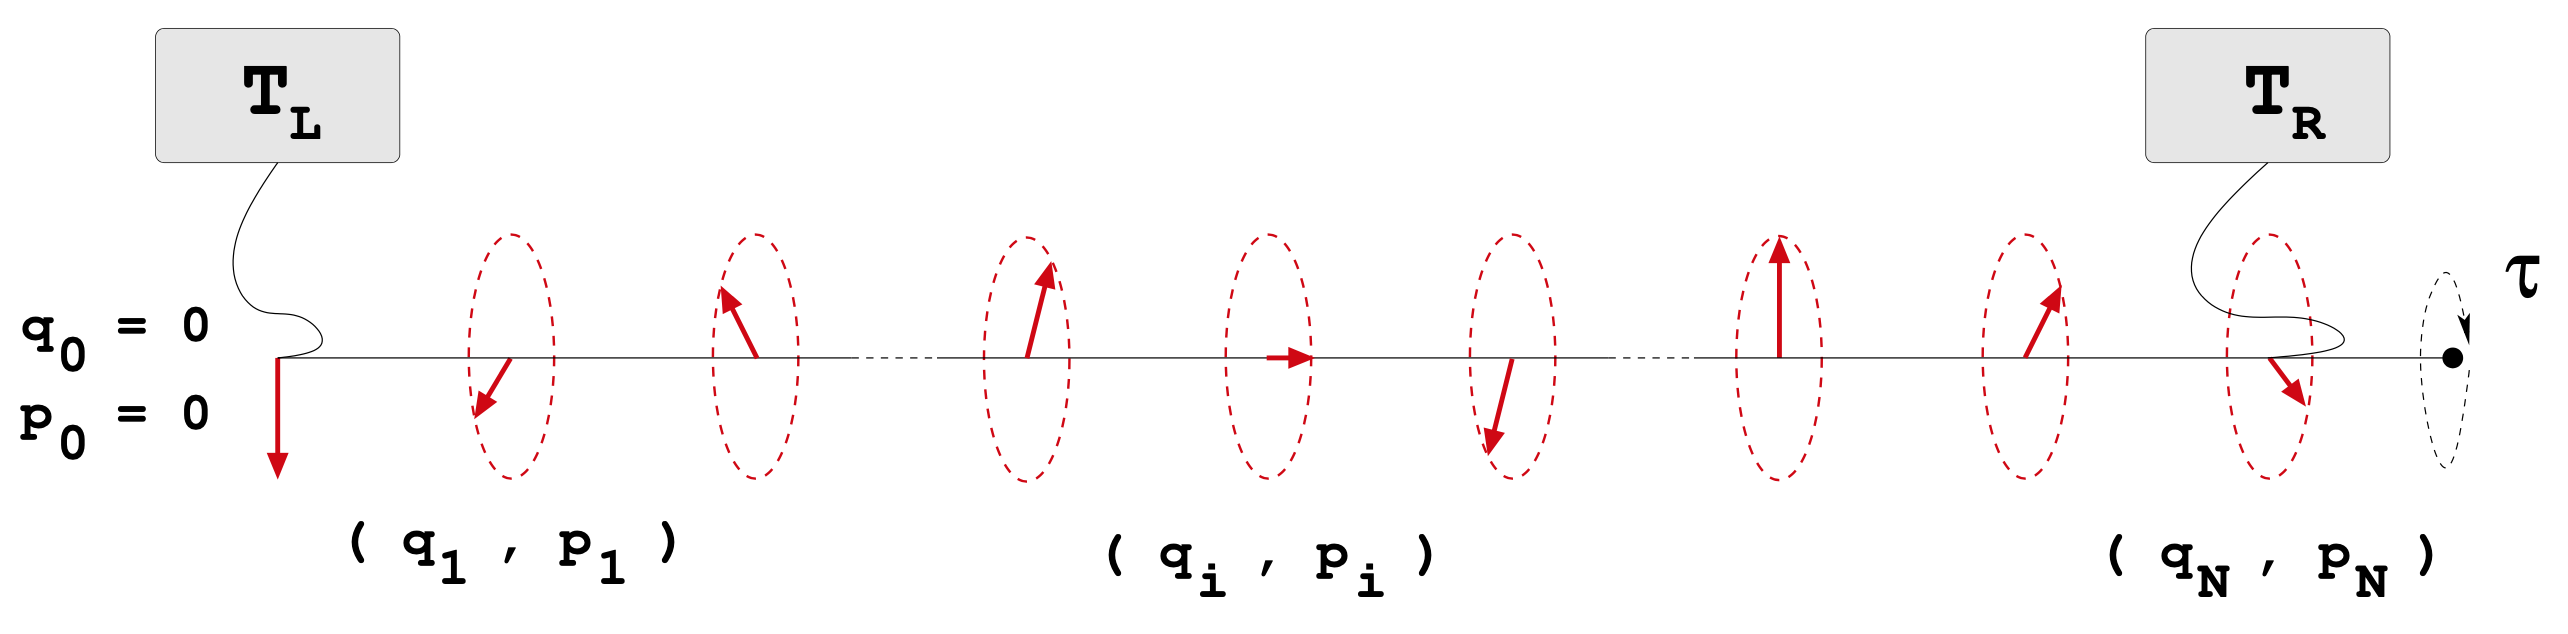
\includegraphics[scale=0.24]{images/rotor_chain.png}
    \end{figure}

    Source : Alessandra Iacobucci, Nonequilibrium stationary states of
    rotor and oscillator chains~\cite{Iacobucci_2011}.

\end{frame}

\begin{frame}

    \frametitle{Modèle - Thermostat de Langevin}

    Un thermostat de Langevin agit comme un bain chauffant.
    Un objet immergé dans un tel bain est
    frappé rapidement par des petites particules, ce qui
    induit un changement de la vitesse (température) de l'objet.
    Par ailleurs, lorsqu'il se déplace, l'objet est restreint
    par les particules du bain, ce qui réduit sa vitesse.

    Ce comportement est un type de fluctuation-dissipation. C'est
    exactement ce qu'on observe dans le mouvement brownien. Un
    grain de pollen immergé dans l'eau, par exemple, est
    poussé par l'agitation thermique des molécules de l'eau, et,
    simultanément, le grain est restreint par la viscosité de l'eau.

\end{frame}

\begin{frame}

    \frametitle{Modèle - Thermostat de Langevin}

    Mathématiquement, un thermostat de Langevin s'exprime alors
    comme la somme de ces 2 forces : celle de la dissipation et celle
    de la fluctuation. Son effet sur le mouvement cinétique est
    donné par
    %
    \[dp = - \gamma p dt + \sigma dW_t,\]
    %
    où $W_t$ est un processus de Wiener standard, et $\sigma$ et $\gamma$
    sont liés par la relation de fluctuation-dissipation :
    \[\sigma^2 = 2 \gamma mkT\]
    %
    Avec $m = k = 1$, on a donc
    \[dp = - \gamma p dt + \sqrt{2 \gamma T_L} dW_t\]

    % The damping factor and the randomforce combine to give the correct canonical ensemble.

\end{frame}


%\begin{frame}
%
%    \frametitle{Modèle - Forçage}
%
%    C'est du type non gradient...
%
%    \colorbox{green}{Ça modelise quoi ?}
%
%    %     % It is precisely because the perturbation is not of gradient type that
%    %    % some particle flux can appear in the steady-state.
%
%\end{frame}


\begin{frame}

    \frametitle{Modèle - Hamiltonien}

    Avec le potentiel $V = \sum_i 1 - \cos(q_i - q_{i-1})$ on
    a le hamiltonien
    %
    \[H(q,p) = \sum_{i=1}^N \left[ \frac{p_i^2}{2}
             + (1 - \cos (q_i - q_{i-1})) \right]\]
    %
    Et les equations de Hamilton,
    \begin{align*}
        dq_i &= p_i dt, \\
        dp_i &= (\sin(q_{i+1} - q_i) - \sin(q_i - q_{i-1}))dt
    \end{align*}


\end{frame}




\begin{frame}

    \frametitle{Modèle - Équations d'évolution}

    En combinant les équations de Hamilton, le forçage $F$, et des
    thermostats de Langevin à gauche et à droite de la chaîne,
    on en tire les équations d'évolution du système :
    %
    \begin{align*}
        dq_i &= p_i dt, \\
        dp_i &= (\sin(q_{i+1} - q_i) - \sin(q_i - q_{i-1}))dt \quad (i \neq 1, N), \\
        dp_1 &= (\sin(q_2 - q_1) - \sin(q_1))dt - \gamma p_1 dt + \sqrt{2 \gamma T_L} dW_t^1, \\
        dp_N &= (F - \sin(q_N - q_{N-1})) dt - \gamma p_N dt + \sqrt{2 \gamma T_R} dW_t^N
    \end{align*}

%    \label{eq:dynamique}

    % Ce qui est précisément la dynamique \eqref{eq:dynamique}.

\end{frame}



    \begin{frame}

    \frametitle{Schéma}

    Moyennant une stratégie de scission (splitting), le schéma
    numérique s'exprime comme une combinaison de l'integration du
    processus d'Ornstein-Uhlenbeck et le schéma de Verlet :
    %
    \begin{align*}
        \tilde p_1^n &= \alpha p_1^n + \sigma_L G_1^n, \\
        \tilde p_N^n &= F + \alpha (p_N^n - F) + \sigma_R G_N^n, \\
        \tilde p_i^n &= p_i^n, i \neq 1,N, \\
        %
        p_i^{n+1/2} &= \tilde p_i^n - \frac{\Delta t}{2}
        \frac{H}{q_i} (q^n, \tilde p^n), \\
        %
        q_i^{n+1} &= q_i^n+ \Delta t p_i^{n+1/2}, \\
        %
        p_i^{n+1} &= p_i^{n+1/2} i - \frac{\Delta t}{2}
        \frac{H}{q_i} (q^{n+1}, p^{n+1/2}),
    \end{align*}
    %
    où $\alpha = e^{-\gamma \Delta t}$,
    $\sigma_L = \sqrt{(1 - \alpha^2)T_L}$,
    et $\sigma_R = \sqrt{(1 - \alpha^2)T_R}$.
    Et $G_1^n$ et $G_1^N$ sont des variables aléatoires gaussiennes.

\end{frame}

\begin{frame}

    \frametitle{Schéma}

    Les 3 premières lignes du schéma constituent l'intégration
    du processus d'Ornstein-Uhlenbeck, qui représente l'influence
    des thermostats et du forçage sur le système. Les thermostats
    n'agissent que sur le premier et le dernier rotor ($i = 1,N$).

    Les 3 dernières lignes constituent le schéma de Verlet, qui
    représente l'évolution Hamiltonienne du système.

    Pour toutes les expériences numériques $\gamma = 1$, et on
    utilise un pas de temps $\Delta t = 0.05$.

\end{frame}





\begin{frame}

    \frametitle{Schéma d'Ornstein-Uhlenbeck}

    Dans les équations d'évolution il y a une partie liée à l'Hamiltonien,
    et une partie stochastique (pour les rotors à gauche et à droite).

    La partie stochastique est le processus d'Ornstein-Uhlenbeck, qui
    s'écrit
    %
    \[dp_t = \theta (\mu - p_t) dt + \sigma dW_t\]
    %
    Pour le rotor à gauche, on a
    $\theta = \gamma$, $\mu = 0$, et $\sigma = \sqrt{2 \gamma T_L}$.
    Pour le rotor à droite, on a
    $\theta = \gamma$, $\mu = F / \gamma$, et $\sigma = \sqrt{2 \gamma T_R}$.

\end{frame}






\begin{frame}

    \frametitle{Schéma d'Ornstein-Uhlenbeck}

    Par la formule d'Itô et la méthode de la variation de la constante,
    la solution du processus d'Ornstein-Uhlenbeck s'écrit
    %
    \[p_t = p_0 e^{-\theta t} + \mu (1 - e^{-\theta t})
    + \sigma \int_0^t e^{-\theta(t-s)} dW_s\]
    %
    Comme l'intégrale d'une fonction déterministe par rapport au mouvement
    brownien est une variable aléatoire gaussienne, $p_t$ est gaussienne.

\end{frame}



\begin{frame}

    \frametitle{Schéma d'Ornstein-Uhlenbeck}

    Moyennant l'isométrie d'Itô, on en tire l'espérance et
    la variance de $p_t$ :
    %
    \[\mathbb{E} [p_t] = p_0 e^{-\theta t} + \mu (1 - e^{-\theta t})\]
    %
    \[\text{Var}(p_t) = \frac{\sigma^2}{2\theta} (1 - e^{-2\theta t})\]
    %
    Donc, sachant la valeur du processus au temps $t$, la valeur du
    processus au temps $t + \Delta t$ est donnée par
    %
    \[p_{t+\Delta t} = p_t e^{-\theta \Delta t} + \mu (1 - e^{-\theta \Delta t})
    + \sigma \sqrt \frac{(1 - e^{-2\theta \Delta t})}{2\theta} G,\]
    %
    où $G$ est une variable aléatoire gaussienne standard.

    % et...... a + \sigma X suit loi normale avec esperance a et
    % variance \sigma^2

\end{frame}



\begin{frame}

    \frametitle{Schéma d'Ornstein-Uhlenbeck}

    Donc, avec $\theta = \gamma$, $\mu = 0$, et
    $\sigma = \sqrt{2 \gamma T_L}$, on a
    %
    \[p_{t+\Delta t} = p_t e^{-\gamma \Delta t}
    + \sqrt{(1 - e^{-2\gamma \Delta t}) T_L} G.\]
    %
    Et avec $\theta = \gamma$, $\mu = F / \gamma$, et
    $\sigma = \sqrt{2 \gamma T_R}$, on a
    %
    \[p_{t+\Delta t} = p_t e^{-\gamma \Delta t}
    + \frac{F}{\gamma} (1 - e^{-\gamma \Delta t})
    \sqrt{(1 - e^{-2\gamma \Delta t}) T_R} G.\]
    %
    Et finalement, avec $\gamma = 1$ et
    $\alpha = e^{-\gamma \Delta t}$, on en tire le schéma
    %
    \begin{align*}
        \tilde p_1^n &= \alpha p_1^n
        + \sqrt{(1 - \alpha^2) T_L} G_1^n, \\
        %
        \tilde p_N^n &= F + \alpha (p_N^n - F)
        + \sqrt{(1 - \alpha^2) T_R} G_N^n
    \end{align*}

\end{frame}












\begin{frame}

    \frametitle{Schéma de Verlet}

    Le schéma de Verlet (ou Störmer-Verlet) est un schéma symplectique
    basé sur une scission de Strang. Le schéma s'exprime comme une composition
    de schémas symplectiques :
    %
    $$\Phi_{\Delta t}^{Verlet} = \phi_{\Delta t/2}^2 \circ \phi_{\Delta t}^1
    \circ \phi_{\Delta t/2}^2,$$
    %
    où $\phi_{\Delta t}^1$ et $\phi_{\Delta t/2}^2$ sont les flux qui
    correspondent aux parties potentielle et cinétique du Hamiltonien :
    %
    $$\phi_{\Delta t}^1 = (q + t M^{-1} p, p)$$
    $$\phi_{\Delta t/2}^2 = (q, p - t\nabla V(q))$$

%    ΦVerlet∆t = φ2∆t/2 ◦ φ1∆t ◦ φ2∆t/2


    % Theorem 2.3.The compositiong◦hof two symplectic mappingsg,h:U→Rnis symplectic
%    Ce qui est symplectique d'après le théorème 2.3 de \cite{stoltz_phys_stat}
    % cheme is time-reversible (in the sense thatS◦ΦVerlet∆t◦S=ΦVerlet−∆t)and symmetric (meaning(ΦVerlet∆t)−1=ΦVerlet−∆t)

\end{frame}





\begin{frame}

    \frametitle{Schéma de Verlet}

    On voit bien que le schéma de Verlet préserve l'énergie. Dans
    ce cas, une chaîne de 1024 rotors a été initialisée avec les
    positions et les impulsions distribuées selon la loi normale
    standard.

    \begin{figure}
        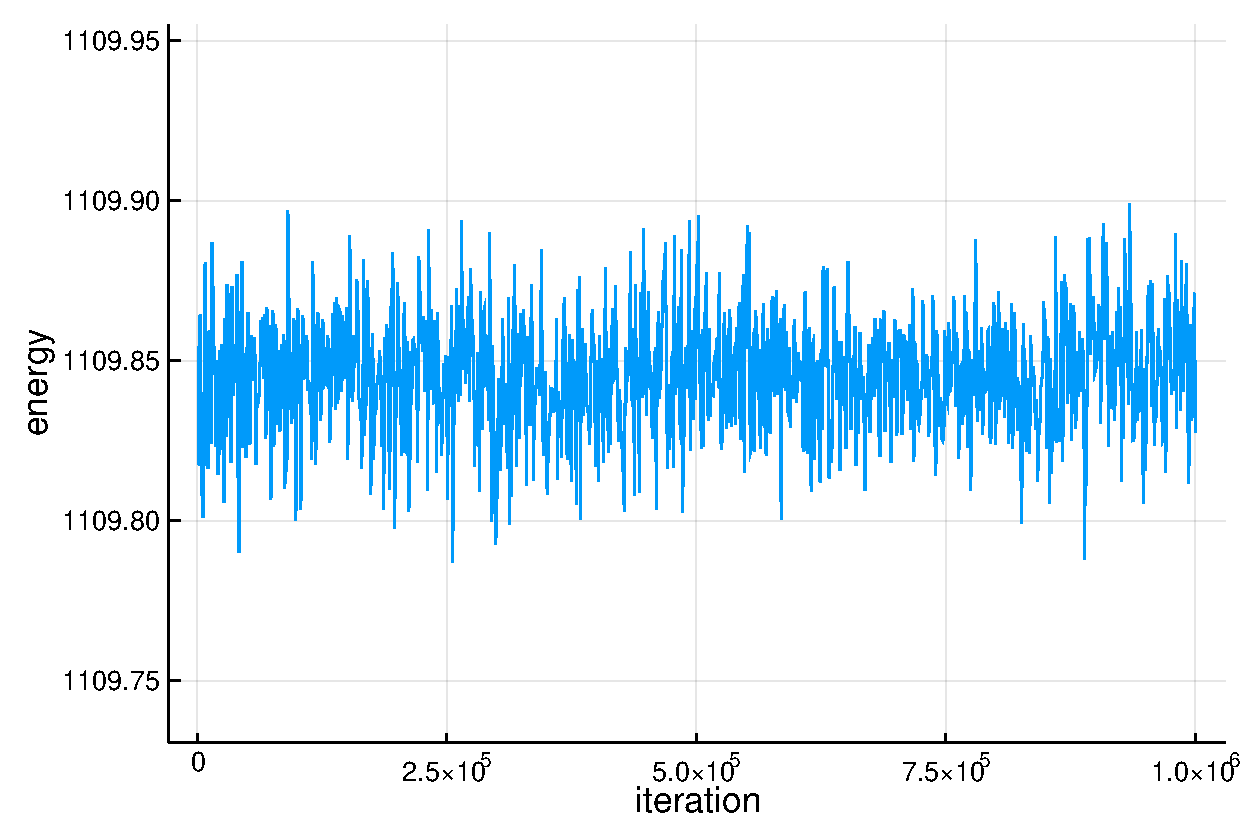
\includegraphics[scale=0.4]{plots/verlet_energy.pdf}
    \end{figure}

\end{frame}

\begin{frame}

    \frametitle{Schéma de Verlet}

    L'écart type de l'énergie croît comme $\Delta t^2$.

    \begin{figure}
        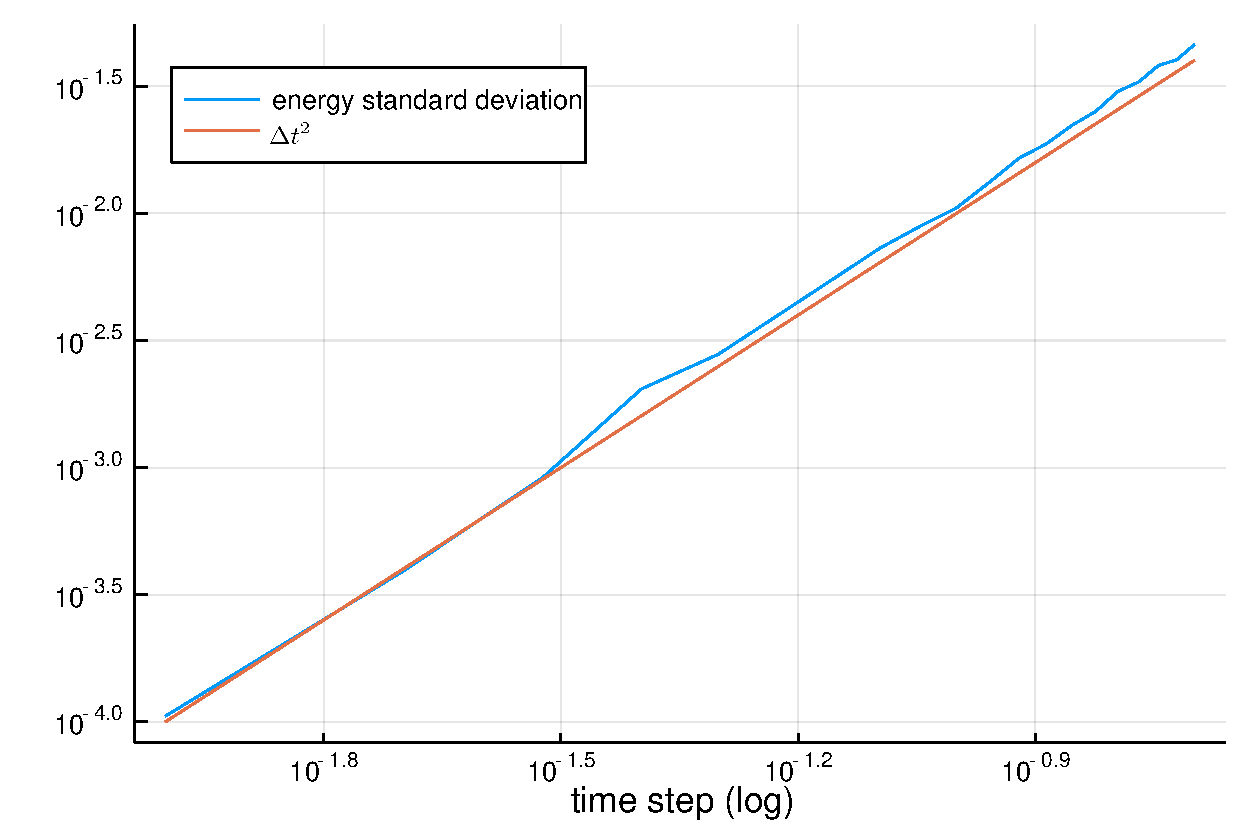
\includegraphics[scale=0.4]{plots/verlet_energy_spread.pdf}
    \end{figure}

\end{frame}


    \begin{frame}

    \frametitle{Température sans forçage}

    Sans forçage, la température varie linéairement pour une faible
    gradient. La variation devient non linéaire pour des gradients
    plus importants car, lorsque le gradient de température est augmenté,
    la conductivité thermique diminue.

    \setlength{\tabcolsep}{2pt}

    \begin{columns}

        \begin{column}{0.8\textwidth}
            \begin{figure}
                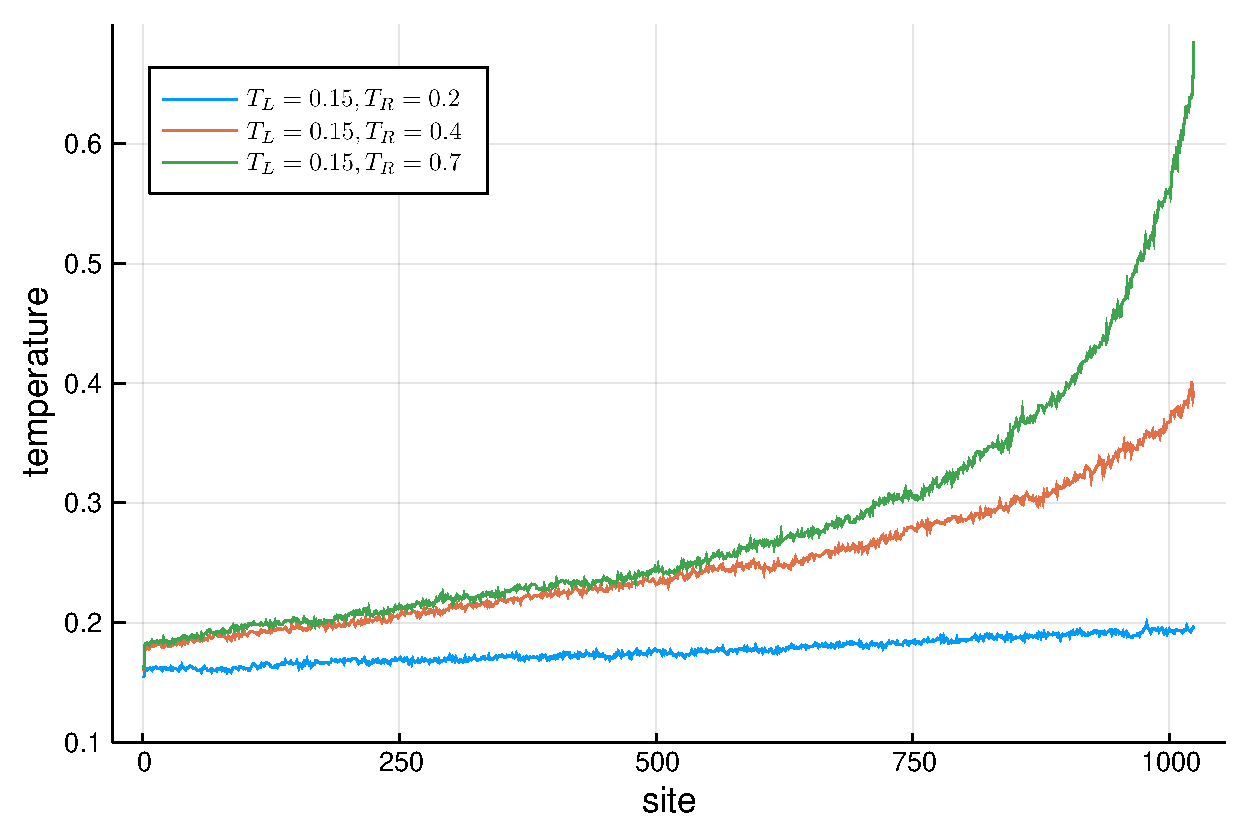
\includegraphics[scale=0.4]{plots/temperature_no_force.pdf}
            \end{figure}
        \end{column}

        \begin{column}{0.20\textwidth}
            \scriptsize
            Rotors : 1024
            Sans forçage
        \end{column}

    \end{columns}

\end{frame}

\begin{frame}

    \frametitle{Température}

    La température est maximum vers le milieu de la chaîne, et
    la position de ce maximum dépend des valeurs des thermostats.

    \begin{columns}

        \begin{column}{0.8\textwidth}
            \begin{figure}
                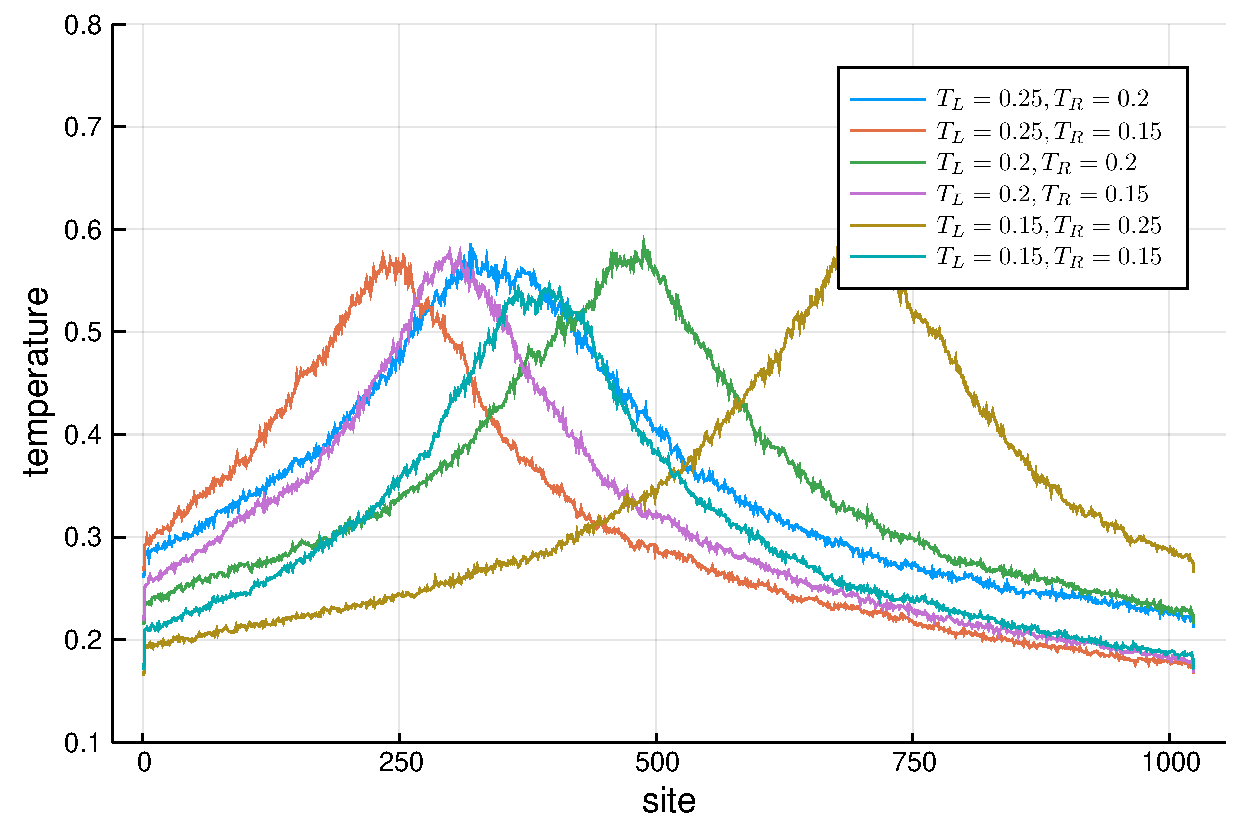
\includegraphics[scale=0.4]{plots/temperature.pdf}
            \end{figure}
        \end{column}

        \begin{column}{0.2\textwidth}
            \scriptsize
            Rotors : 1024
            Forçage : 1.6
        \end{column}

    \end{columns}

\end{frame}

\begin{frame}

    \frametitle{Impulsion Moyenne}

    Le profil de l'impulsion moyenne n'est pas linéaire, et la
    position de sa dérivée maximale coïncide avec la position de
    la température maximale.

    \begin{columns}

        \begin{column}{0.8\textwidth}
            \begin{figure}
                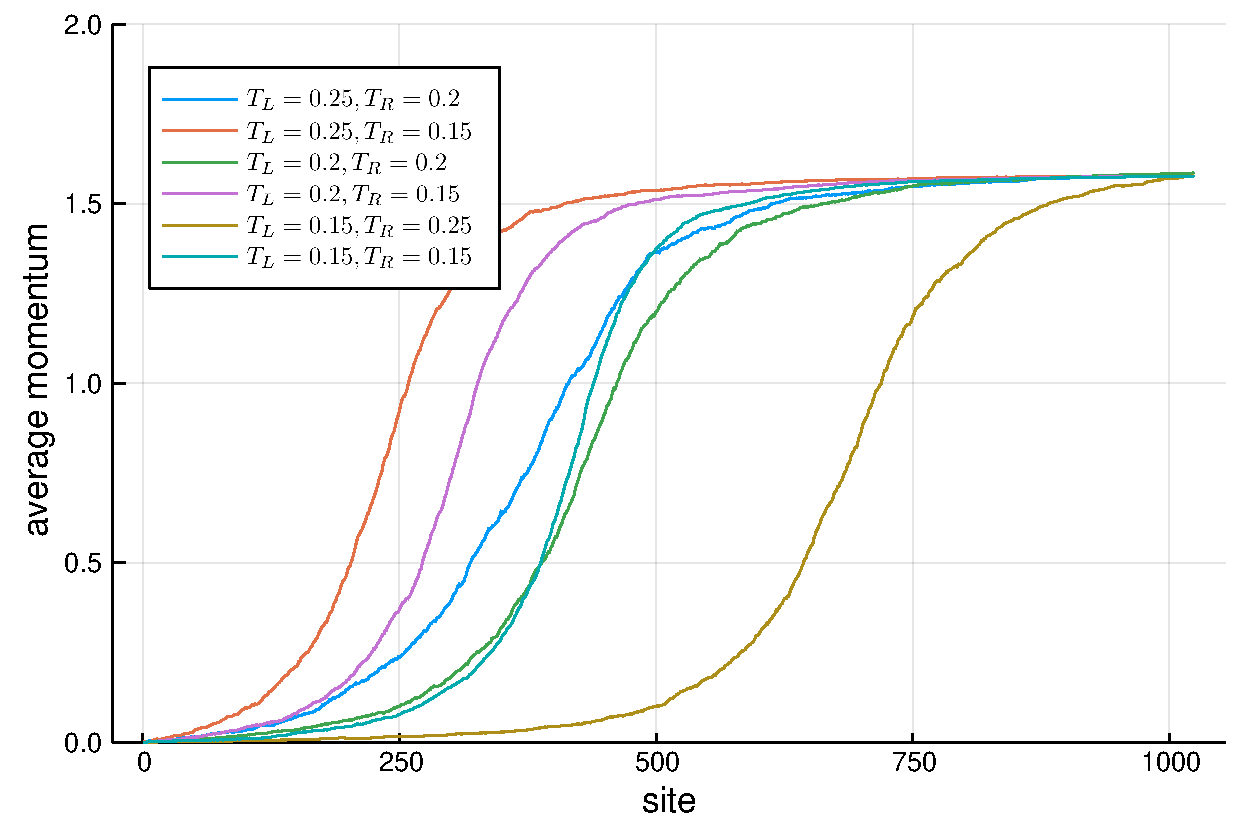
\includegraphics[scale=0.4]{plots/average_momentum.pdf}
            \end{figure}
        \end{column}

        \begin{column}{0.2\textwidth}
            \scriptsize
            Rotors : 1024
            Forçage : 1.6
        \end{column}

    \end{columns}

\end{frame}

\begin{frame}

    \frametitle{Impulsion Moyenne}

    L'impulsion moyenne pour des chaînes de longueurs différentes
    sur la même échelle.

    \begin{columns}

        \begin{column}{0.8\textwidth}
            \begin{figure}
                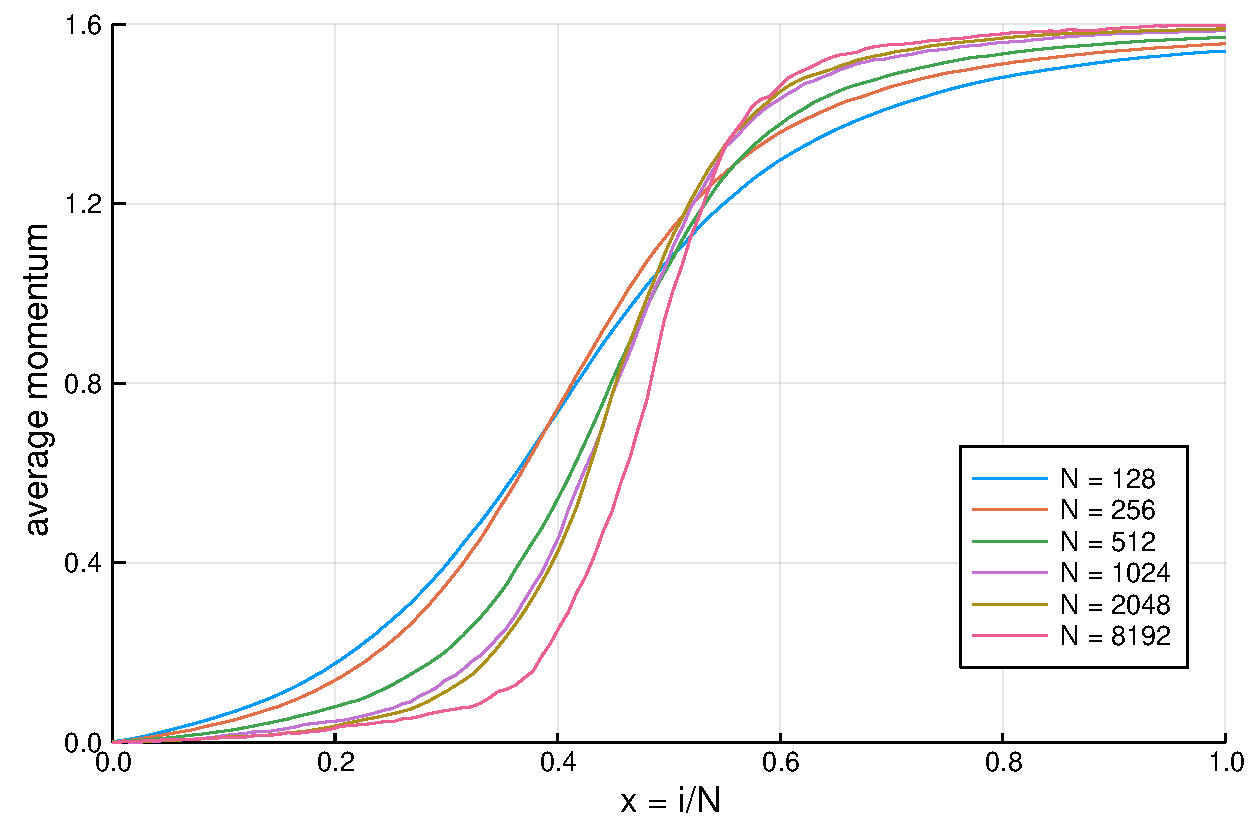
\includegraphics[scale=0.4]{plots/average_momentum_scaled.pdf}
            \end{figure}
        \end{column}

        \begin{column}{0.2\textwidth}
            \scriptsize
            Forçage : 1.6 \\
            $T_L$ : 0.2 \\
            $T_R$ : 0.2
        \end{column}

    \end{columns}

\end{frame}

\begin{frame}

    \frametitle{Température cinétique et potentielle}

    Pour les chaînes les plus longues on a l'accord entre la
    température cinétique (lignes solides) et la température
    potentielle.

    \begin{columns}

        \begin{column}{0.8\textwidth}
            \begin{figure}
                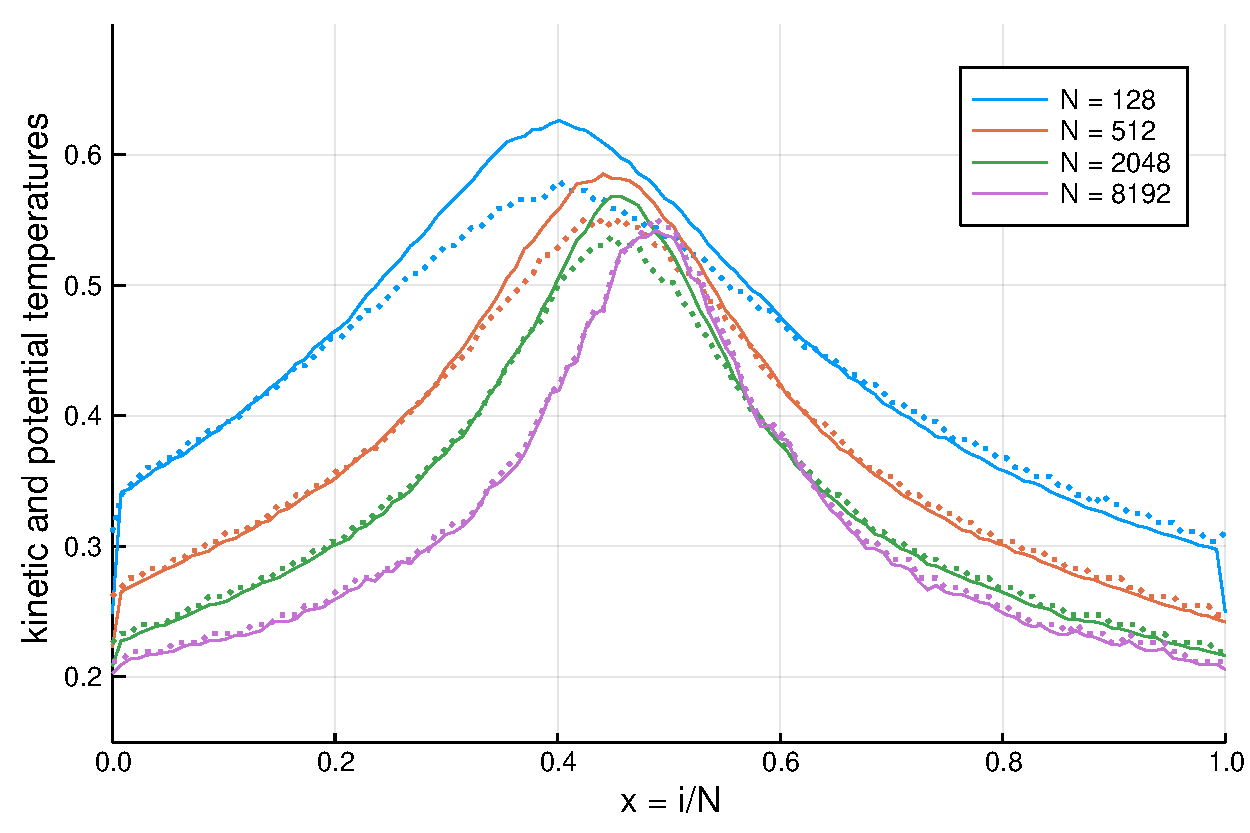
\includegraphics[scale=0.4]{plots/temperature_scaled.pdf}
            \end{figure}
        \end{column}

        \begin{column}{0.2\textwidth}
            \scriptsize
            Cinétique : \\
            ligne solide \\
            \vspace{3mm}
            Potentielle : \\
            ligne pointillée

        \end{column}

    \end{columns}

\end{frame}

\begin{frame}

    \frametitle{Distribution de l'impulsion}

    Distribution empirique de l'impulsion du rotor le plus chaud,
    et la distribution de Gibbs :
    $Z_\text{kin}^{-1} \exp[-(p - \overline p_i)^2 / (2T_i)]$,
    où $i$ est l'index du rotor le plus chaud et
    $Z_\text{kin} = \sqrt{2 \pi T_i}$.

    \begin{columns}

        \begin{column}{0.8\textwidth}
            \begin{figure}
                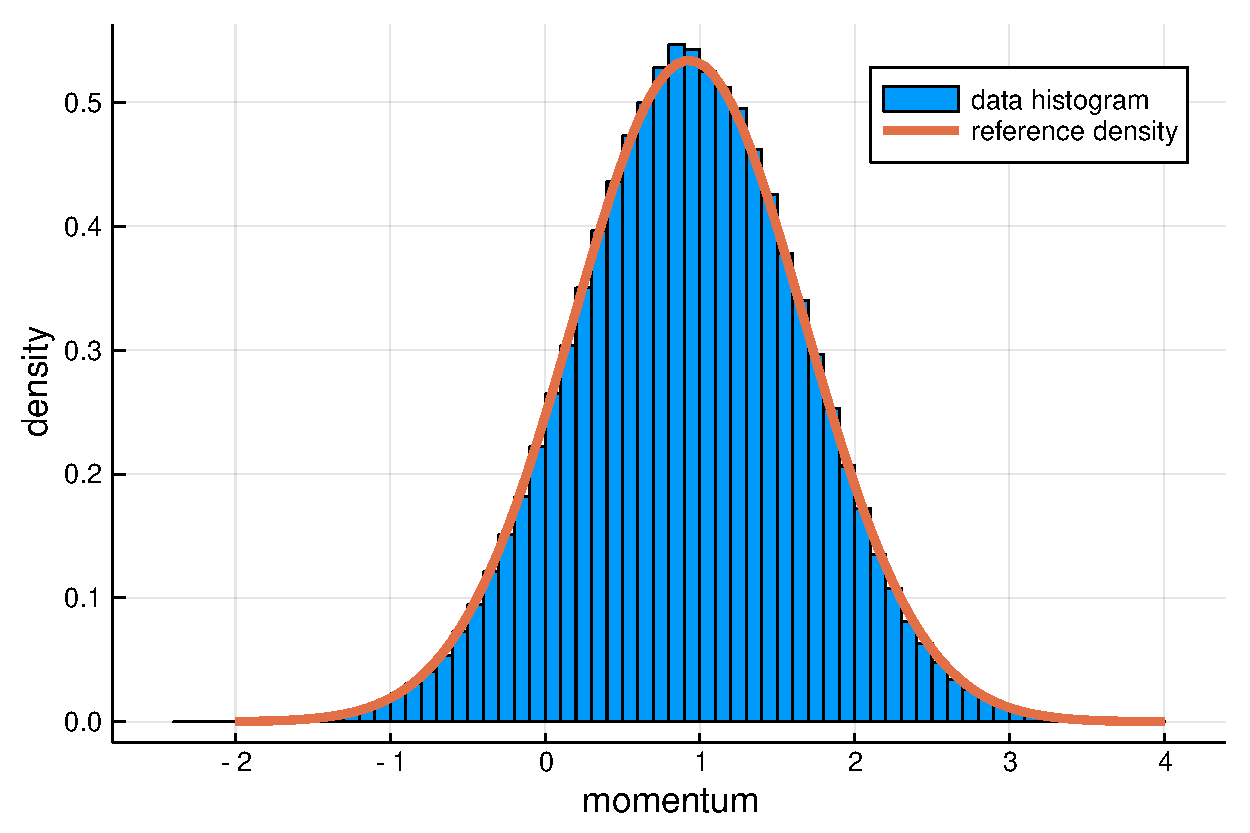
\includegraphics[scale=0.4]{plots/gibbs_momentum.pdf}
            \end{figure}
        \end{column}

        \begin{column}{0.2\textwidth}
            \scriptsize
            Rotors : 1024
            Forçage : 1.6
            $T_L = T_R = 0.2$
        \end{column}

    \end{columns}

\end{frame}

\begin{frame}

    \frametitle{Distribution de la distance}

    Distribution empirique de la distance du rotor le plus chaud
    (à son voisin), et la distribution de Gibbs :
    $Z_\text{pot}^{-1} \exp[-V(r) / T_i]$,
    où $i$ est l'index du rotor le plus chaud.
%    et $Z_\text{pot}$ est calculé.

    \begin{columns}

        \begin{column}{0.8\textwidth}
            \begin{figure}
                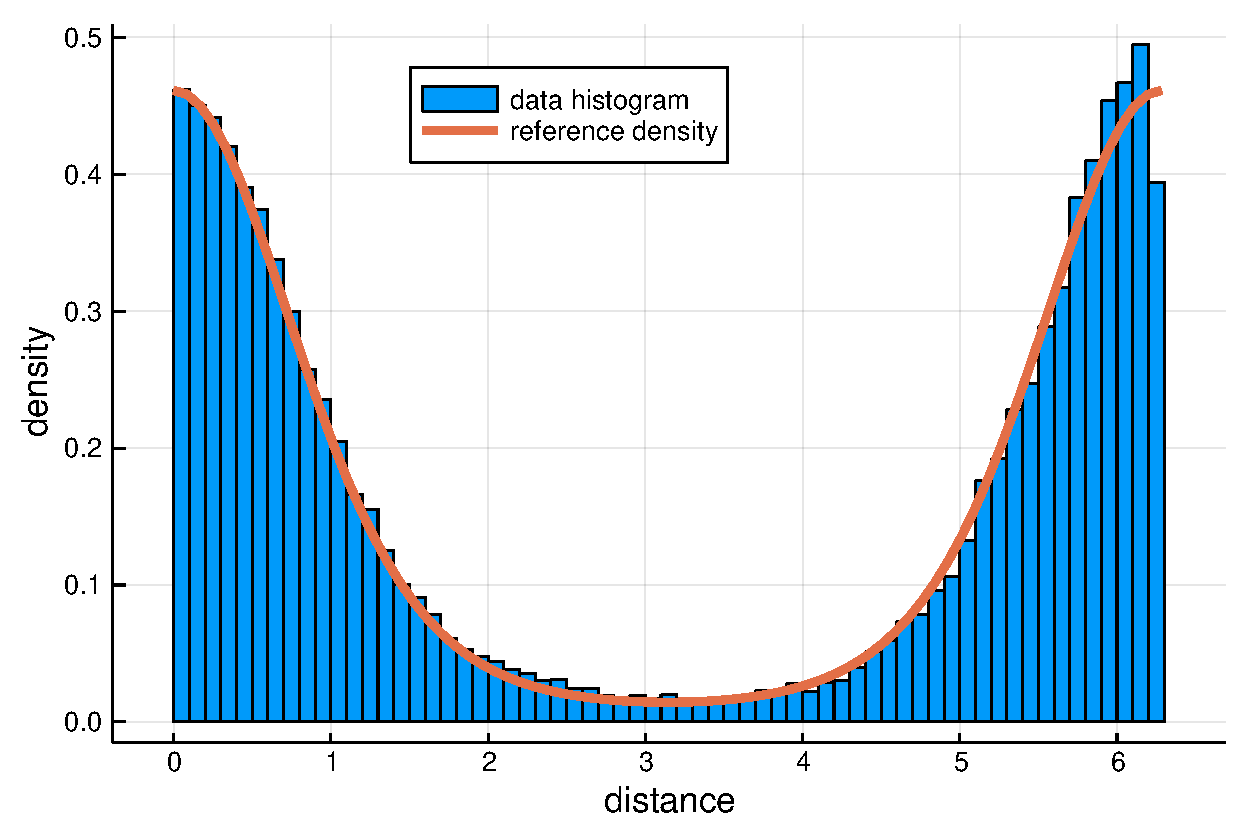
\includegraphics[scale=0.4]{plots/gibbs_distance.pdf}
            \end{figure}
        \end{column}

        \begin{column}{0.2\textwidth}
            \scriptsize
            Rotors : 1024
            Forçage : 1.6
            $T_L = T_R = 0.2$
        \end{column}

    \end{columns}

\end{frame}

\begin{frame}

    \frametitle{Indépendance des impulsions et distances}

    Décroissance de l'erreur par rapport au nombre d'échantillons
    entre la distribution jointe et le produit tensoriel des
    impulsions et des distances.
    %
    $\delta_n = \int_{[0,2\pi] \times \mathbb{R}} |\psi^n(r,p)
    - \overline \psi^n(r) \overline \psi^n(p)]| dr dp.$

    \begin{columns}

        \begin{column}{0.8\textwidth}
            \begin{figure}
                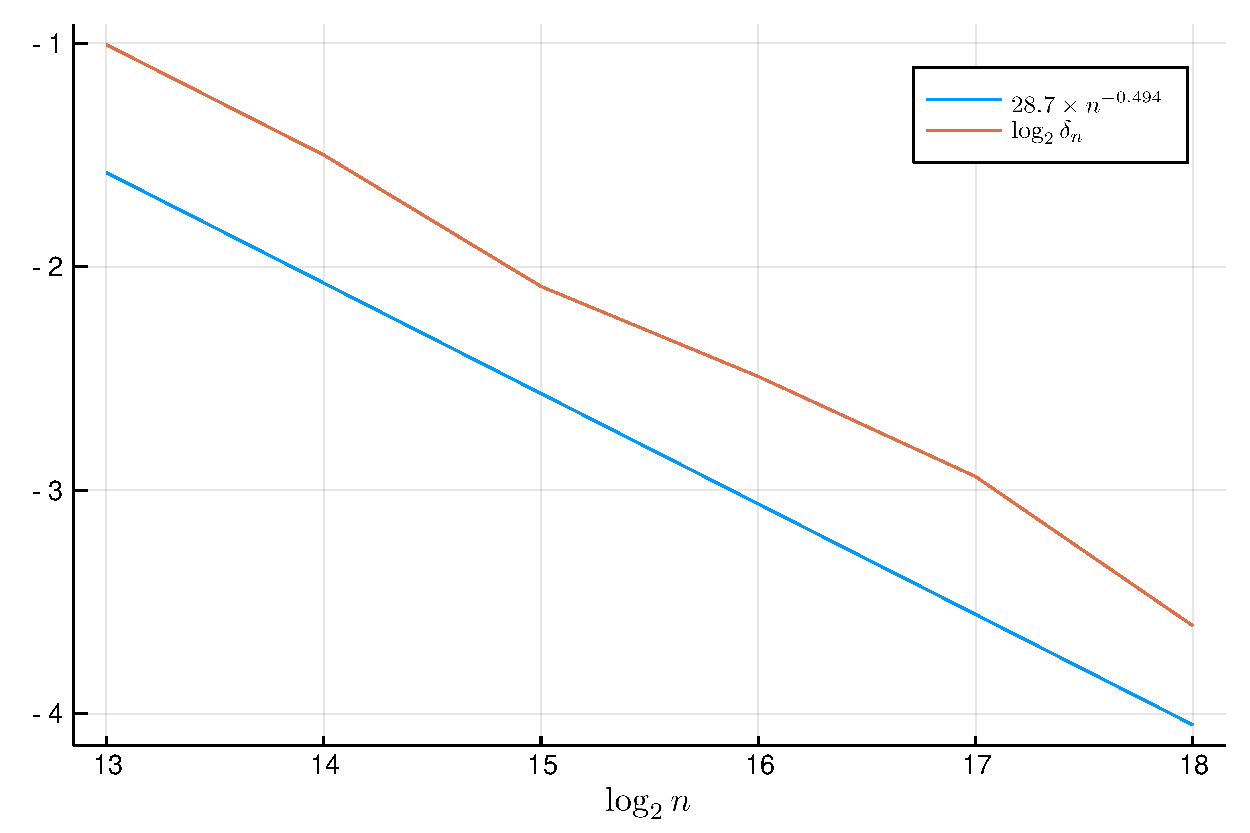
\includegraphics[scale=0.4]{plots/distribution_error.pdf}
            \end{figure}
        \end{column}

        \begin{column}{0.2\textwidth}
            \scriptsize
            Rotors : 1024
            Forçage : 1.6
            $T_L = T_R = 0.2$

            \vspace{2.0mm}

            Décroissement :
            $\delta_n \approx 13 \times n^{-0.491}$

        \end{column}

    \end{columns}

\end{frame}

\begin{frame}

    \frametitle{Flux d'énergie normal}

    Le flux d'énergie par rapport au forçage pour des chaînes de longueurs
    différentes. La température à droite est 0.15. La couleur des courbes
    indique la température á gauche (0.15, 0.2, et 0.25).

    \begin{columns}

        \begin{column}{0.8\textwidth}
            \begin{figure}
                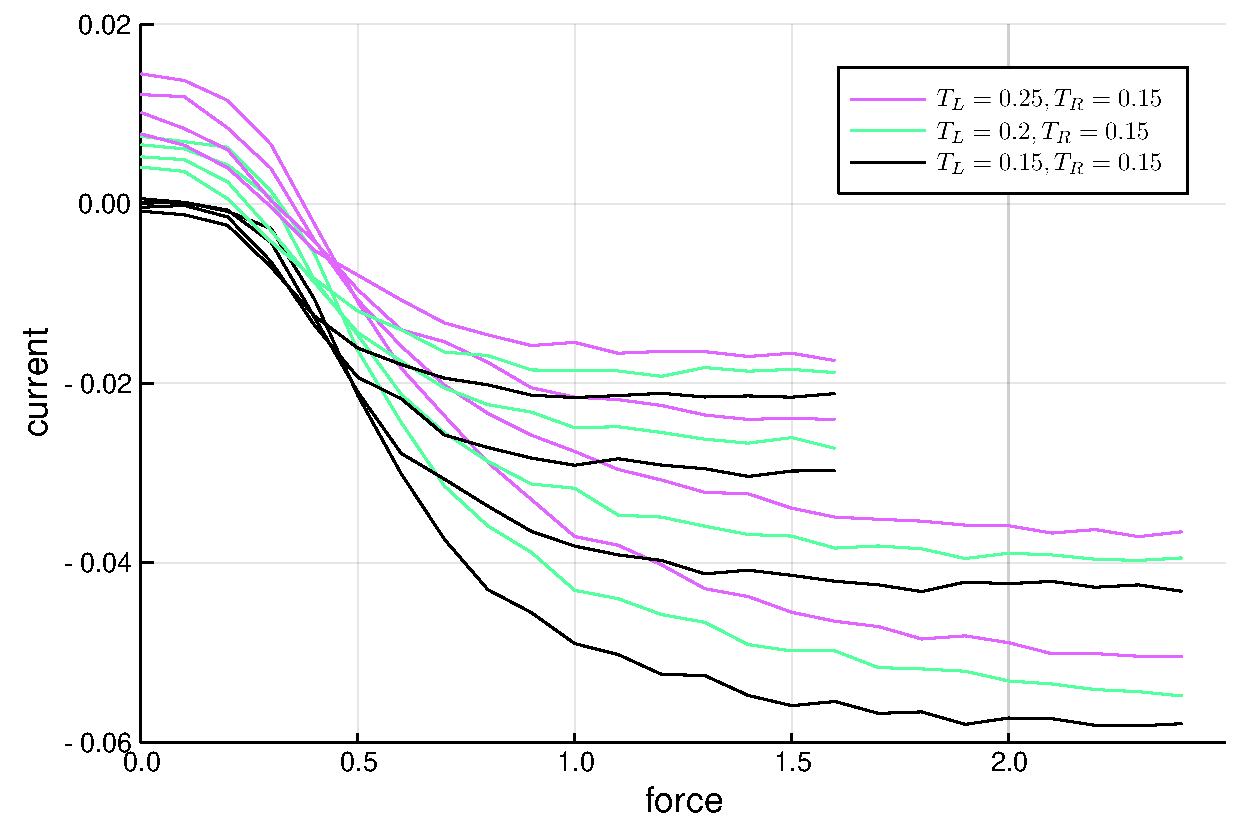
\includegraphics[scale=0.4]{plots/energy_current_normal.pdf}
            \end{figure}
        \end{column}

        \begin{column}{0.2\textwidth}

            \scriptsize

            \vspace{18.0mm}
            N = 1024

            \vspace{3.0mm}
            N = 512

            \vspace{4.0mm}
            N = 256

            \vspace{5.0mm}
            N = 128

        \end{column}

    \end{columns}

\end{frame}

\begin{frame}

    \frametitle{Flux d'énergie étrange}

    Ici, la réduction de la température à droite suscite une
    \alert{augmentation} du courant vers la gauche. Une explication est
    que la réduction de température augmente la conductivité, et donc
    le forçage a davantage d'influence sur le système.

    \begin{columns}

        \begin{column}{0.8\textwidth}
            \begin{figure}
                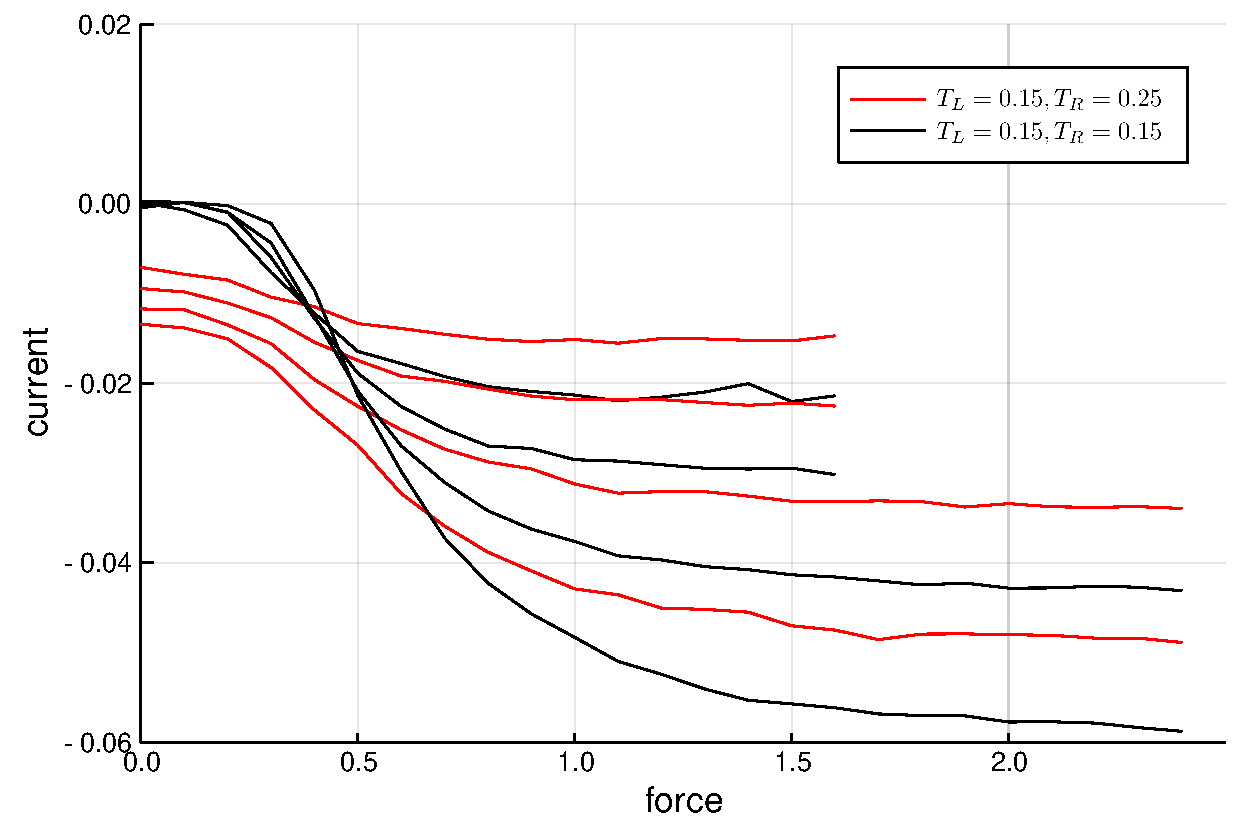
\includegraphics[scale=0.4]{plots/energy_current_strange.pdf}
            \end{figure}
        \end{column}

        \begin{column}{0.2\textwidth}

            \scriptsize

            \vspace{15.0mm}
            N = 1024

            \vspace{3.0mm}
            N = 512

            \vspace{4.0mm}
            N = 256

            \vspace{5.0mm}
            N = 128

        \end{column}

    \end{columns}

\end{frame}


    \begin{frame}
        \center \Huge Merci !
    \end{frame}

    \begin{frame}[allowframebreaks]

        \frametitle{Références}

        \renewcommand*{\bibfont}{\scriptsize}
        \nocite{*}
        \printbibliography[title=All]

    \end{frame}

\end{document}
